\section{Results and Discussions}
\subsection{Missingness MAR Validity}

The validity of applying imputation techniques like VAE hinges on the nature of the missing data. We formally tested the hypothesis that missingness in key personal variables (\texttt{height\_cm}, \texttt{age}, \texttt{gender}, \texttt{weight\_kg}) was dependent on other observed variables, thereby providing evidence against the MCAR assumption. Univariate tests (Chi-squared, t-tests) and multivariate logistic regressions were employed. The results, originally presented in detail in Table~\ref{tab:MAR_Summary}, consistently showed statistically significant associations ($p < 0.05$) between missingness and observed predictors. The logistic regression models achieved high predictability for missingness in height (AUC = 0.969), age (AUC = 0.984), and weight (AUC = 0.976). While the AUC for gender was lower, significant univariate associations remained. Table~\ref{tab:MAR_Summary} provides a condensed overview of these findings.

Based on domain knowledge of the data collection process, where data represent experimental records aggregated from various contributors, missingness often occurred systematically within specific experimental groups (defined by characteristics such as contributor, location, or building type, aligning with the statistical associations found). This typically reflected a determination by the data contributor at the time of the experiment that recording a specific variable was not required or relevant for that particular experimental condition or protocol. While the possibility that missingness could, in some cases, be related to the unobserved value itself (MNAR) cannot be entirely excluded without more granular information on the exact reason for each missing entry, the observed systematic patterns linked to recorded experimental factors lend stronger support to the MAR assumption. Therefore, we proceeded under the MAR assumption for VAE imputation, acknowledging this as a standard, necessary assumption for applying such imputation techniques in complex observational datasets\cite{Rubin1976}.

\begin{table}[htbp]
    \centering
    \caption{Simplified Summary of MAR Validation Results}
    \label{tab:MAR_Summary}
    \begin{tabular}{l l l}
        \toprule
        Variable & Key Evidence Finding & Overall Assessment (vs. MCAR) \\
        \midrule
        Height (\texttt{height\_cm}) & Multiple Sig. Assoc.; High AUC (0.969) & Evidence against MCAR \\
        Age (\texttt{age}) & Multiple Sig. Assoc.; High AUC (0.984) & Evidence against MCAR \\
        Gender (\texttt{gender}) & Multiple Sig. Assoc.; Low/Mod AUC (0.673) & Evidence against MCAR \\
        Weight (\texttt{weight\_kg}) & Multiple Sig. Assoc.; High AUC (0.976) & Evidence against MCAR \\
        \bottomrule
    \end{tabular}
    \vspace{1ex} % Add some space below the table
    \footnotesize % Smaller font for the note
    Note: Summarizes statistical tests (Chi-squared, t-tests, logistic regression AUC) assessing dependency of missingness on observed variables. Significant findings support MAR/MNAR over MCAR.
\end{table}

These results strongly suggest that the missing data mechanism is consistent with MAR or potentially Missing Not At Random (MNAR). Given the data collection context (aggregation from various experiments), systematic missingness linked to specific protocols or contributor choices aligns well with the MAR assumption. Therefore, we proceeded with VAE-based imputation under the MAR assumption, acknowledging it as a standard and necessary premise for applying such techniques to complex observational datasets \cite{Rubin1976}. Therefore, despite the potential for MNAR in some fields, the dominant missingness patterns are consistent with MAR, justifying the use of VAE-based imputation.


\subsection{BMR Ablation Results}
First and foremost, examining the aggregated out-of-sample lightgbm models performance on the BMRs (calculated only when inputs are available), we were able to calculate their respective relative RMSE, MAE and MAPE as according to Figure~\ref{fig:lightgbm-bmrs}. Across the three heat maps, the top rows are where the overall data availability is better, and towards the bottom the data availability becomes worse. The BMR models yielded consistent improvements across the board with data fill above 80\% when evaluating against RMSe and MAE, and starts to see a variation of performance, where Livingston–Kohlstadt appears to have the best performance across the three models, which is to be expected since it is a much newer calculation approach compared to the other two. It is also worth noticing that when the level of data fill falls below 50\%, all but the Livingston-Kohlstadt variant started to consistently show deterioration of performance, which is to be anticipated since the model's performance improvement now requires more inputs from BMR fields than before. %This is strangely put, revise later.
\begin{figure}[h!]
    \centering
    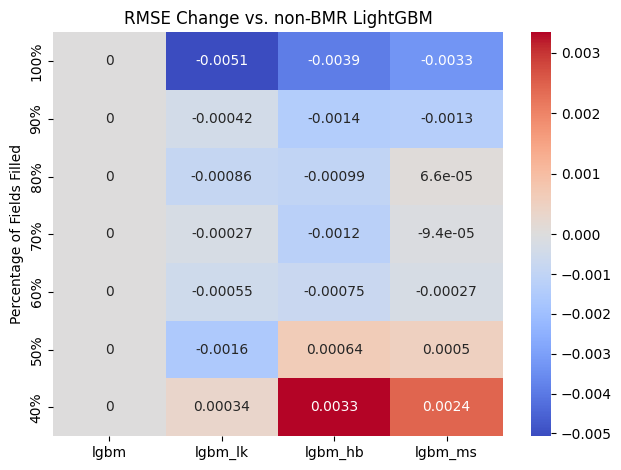
\includegraphics[width=0.3\linewidth]{fig/lgbrmse.png}
    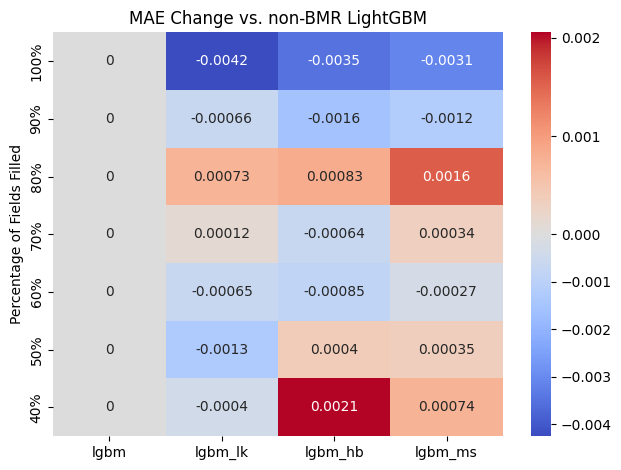
\includegraphics[width=0.3\linewidth]{fig/lgbmae.png}
    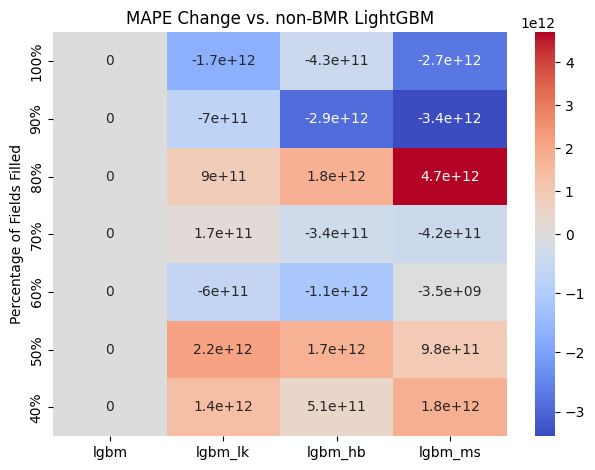
\includegraphics[width=0.3\linewidth]{fig/lgbmape.png}
    \caption{Relative RMSE, MAE and MAPE of lightgbm models trained with different BMR equations}
    \label{fig:lightgbm-bmrs}
\end{figure}

% This translates to ? \% of overall RMSE improvement towards the lightgbm model simply by engineering BMR terms - which is inherently an analytical-equation-driven feature engineering exercise. Yet by working with this one variable only we believe we have demonstrated how adding additional analytically-described features that are truly transformed existing inputs can have the effect of improving the performance of thermal sensation predictor. 

The inclusion of calculated Basal Metabolic Rate (BMR) as an input feature demonstrated tangible benefits for the LightGBM benchmark model. As highlighted previously, the addition of BMR features, particularly leveraging the Livingston-Kohlstadt formulation \cite{LivingstonKohlstadt2005}, yielded an overall performance improvement of approximately 8\% in predictive accuracy (based on RMSE/MAE metrics, see Highlights) compared to the identical LightGBM model trained without BMR inputs. This underscores the value of incorporating physiology-based, analytically derived features, even when based on inputs (age, height, weight) that themselves suffer from missingness, for improving thermal sensation prediction. The Livingston-Kohlstadt variant generally provided the most consistent benefits, particularly in data subsets with higher completeness (fill > 80\%), although performance gains diminished or reversed in highly incomplete data (fill < 50\%), likely due to the unreliability of BMR inputs in those cases.


\subsection{Performance Evaluation}
\subsubsection{Thermal Sensation Prediction: Overall Performance Evaluation}
The performance of the baseline model (\texttt{pmv\_ce}), the benchmark (lightgbm), and the sequentially developed models (vae, \texttt{pv\_pen}, \texttt{pvp\_pen}, ultra) were evaluated using RMSE, MAE, MAPE, SMAPE, and $R^2$ metrics. The results are summarized in Table \ref{tab:performance_updated}.

\begin{table}[h!] % You can adjust the placement specifier [htbp] as needed
\centering
\caption{Overall Model Performance Comparison} % Add your desired caption
\label{tab:performance_updated} % Add a label for referencing
\begin{tabular}{lcccccc}
\toprule
Metric/Model & pmv\_ce & lightgbm & vae     & pv\_pen & pvp\_pen & ultra  \\
\midrule
RMSE   & 1.310   & 0.952    & 1.205   & 0.994   & 0.991    & 0.984  \\
MAE    & 1.001   & 0.711    & 0.880   & 0.745   & 0.745    & 0.739  \\
MAPE   & 101.7\% & 76.3\%   & 99.6\%  & 80.9\%  & 80.6\%   & 79.8\% \\
SMAPE  & 154.2\% & 145.8\%  & 185.3\% & 153.7\% & 152.5\%  & 149.8\%\\
$R^2$     & -0.185  & 0.376    & 0.000   & 0.320   & 0.324    & 0.334  \\
\bottomrule
\end{tabular}
\end{table}
The \texttt{pmv\_ce} baseline exhibited the poorest performance across all metrics, notably yielding a negative $R^2$ value (-0.185). The lightgbm benchmark, which handled missing data internally, achieved the lowest RMSE (0.952) and MAE (0.711), and the highest $R^2$ (0.376). The standard \gls{vaeplain} model performed poorly, with high errors (e.g., SMAPE 185.3\%) and an $R^2$ of 0.000. LightGBM's superior overall RMSE/MAE metrics might stem from its capacity to capture highly complex, non-linear interactions within the full feature set, potentially including latent patterns derived implicitly from the missing data itself. While effective for raw prediction, this contrasts with the PINN-VAE approach, where the VAE structure and explicit physiological constraints may introduce beneficial regularization and interpretability at the cost of potentially smoothing over some intricate data patterns.

Introducing physics-informed constraints (\texttt{pv\_pen}) significantly improved upon the vae, reducing RMSE from 1.205 to 0.994 and increasing $R^2$ from 0.000 to 0.320. Further incorporating personalization (\texttt{pvp\_pen}) resulted in marginal improvements over \texttt{pv\_pen}, with RMSE decreasing to 0.991 and $R^2$ increasing to 0.324. The \gls{ultra} model, using imputed data with LightGBM, performed slightly worse than the lightgbm benchmark that handled missingness implicitly (RMSE 0.984 vs 0.952; $R^2$ 0.334 vs 0.376).

The results indicate that the standard PMV-based model (\texttt{pmv\_ce}) is insufficient for accurately predicting thermal sensation in the extent of dataset this large. The LightGBM benchmark (lightgbm) demonstrated strong predictive power, achieving the best overall metrics by effectively leveraging the dataset, including missing values.

However, while lightgbm's performance is high, its internal mechanisms for handling missingness operate essentially as a "black box". The model may learn predictive patterns from the presence of missing data itself, but this does not necessarily translate into actionable or interpretable insights. For instance, superior performance relying on missingness patterns does not yield practical recommendations like "ensure this data point remains missing for better comfort prediction". This inherent limitation in interpretability regarding missing data motivates the development of models that aim for a more structured or causal understanding, even if benchmark metrics are slightly lower.

A detailed feature importance analysis (e.g., using SHAPley values or permutation importance) for the LightGBM model was not conducted as part of this study. LightGBM primarily served as a high-performance benchmark, establishing a reference point for predictive accuracy attainable by a state-of-the-art gradient boosting model that handles missing data implicitly. The focus of our analysis was on comparing the performance and characteristics of the explicitly constrained PINN-VAE approaches against this benchmark, rather than performing an in-depth feature attribution analysis of the benchmark model itself.

\begin{figure}[h!]
    \centering
    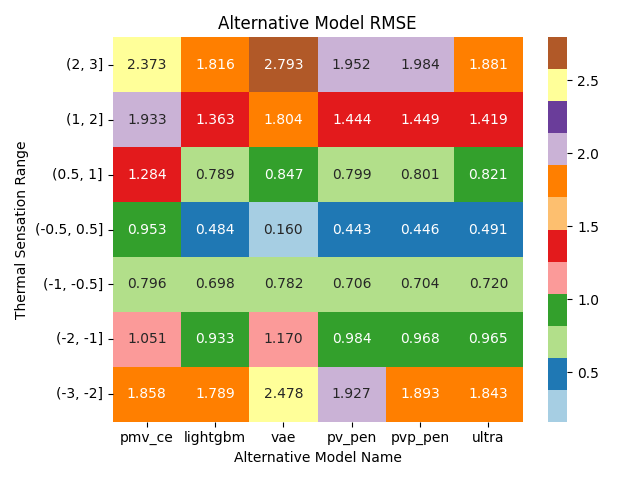
\includegraphics[width=0.5\linewidth]{fig/rmse_all_7.png}
    \caption{Alternative Model RMSEs across thermal sensation buckets}
    \label{fig:rmse-7bucket}
\end{figure}

The poor performance of the standard VAE (vae) highlights the challenges of applying generative models directly without domain constraints. Attempting to impute the missing values during the 5-fold epochs, the trained VAE ended up predicting all predictions as positive values, leading to not only a $R^2$ score at 0, but also an unusable model. In contrast, the substantial improvement observed as in Figure~\ref{fig:rmse-7bucket} with the PINN-VAE (\texttt{pv\_pen}) the significant benefit of integrating physics-informed constraints when performing parallel training of model alongside missing data imputation. This step aligns the model more closely with underlying physical principles and brought its performance much closer to the lightgbm benchmark, particularly in explained variance ($R^2$).

The addition of personal physiological indices (\texttt{pvp\_pen}) provided further, albeit smaller, performance gains, validating the hypothesis that personalization can enhance prediction accuracy within this physically-constrained framework. Comparing ultra and lightgbm, the results suggest that for this particular dataset and imputation strategy, allowing LightGBM to handle missing data internally was more advantageous than the explicit imputation method employed.

Overall, there is a potential trade-off: the lightgbm benchmark offers peak predictive accuracy by leveraging all patterns including missingness, but with limited interpretability regarding why missingness might be predictive. The PINN-VAE approaches (\texttt{pv\_pen}, \texttt{pvp\_pen}), while achieving slightly lower metrics in this instance, represent a promising pathway for integrating domain knowledge and personalization, potentially offering more interpretable and structurally sound predictions for thermal sensation.
% \begin{figure}[h!]
%     \centering
%     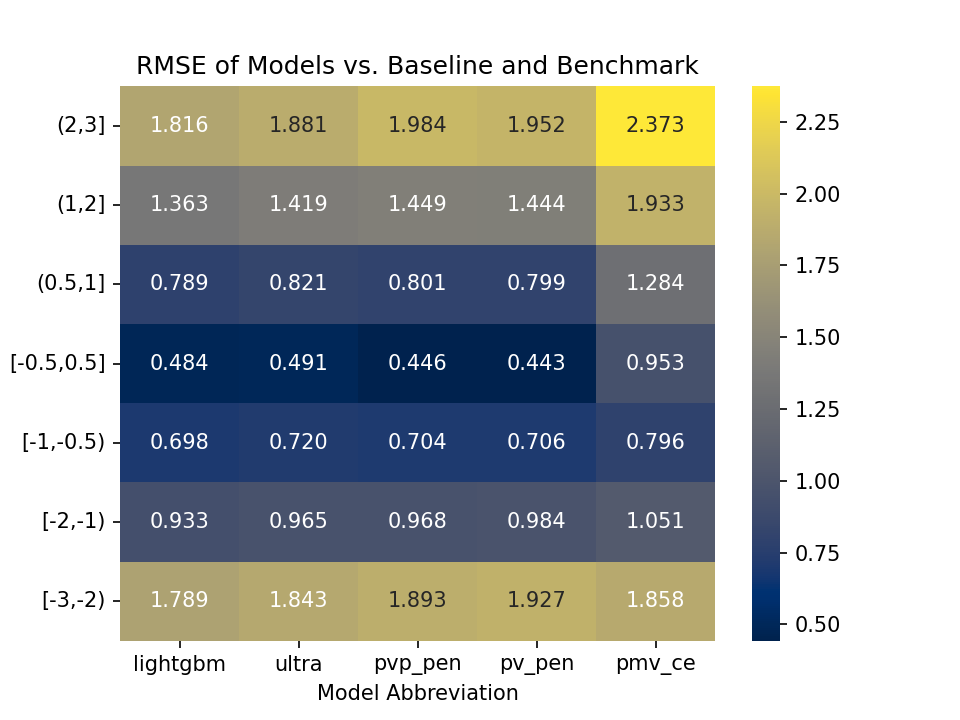
\includegraphics[width=0.49\linewidth]{fig/mods_rmse_hm.png}
%     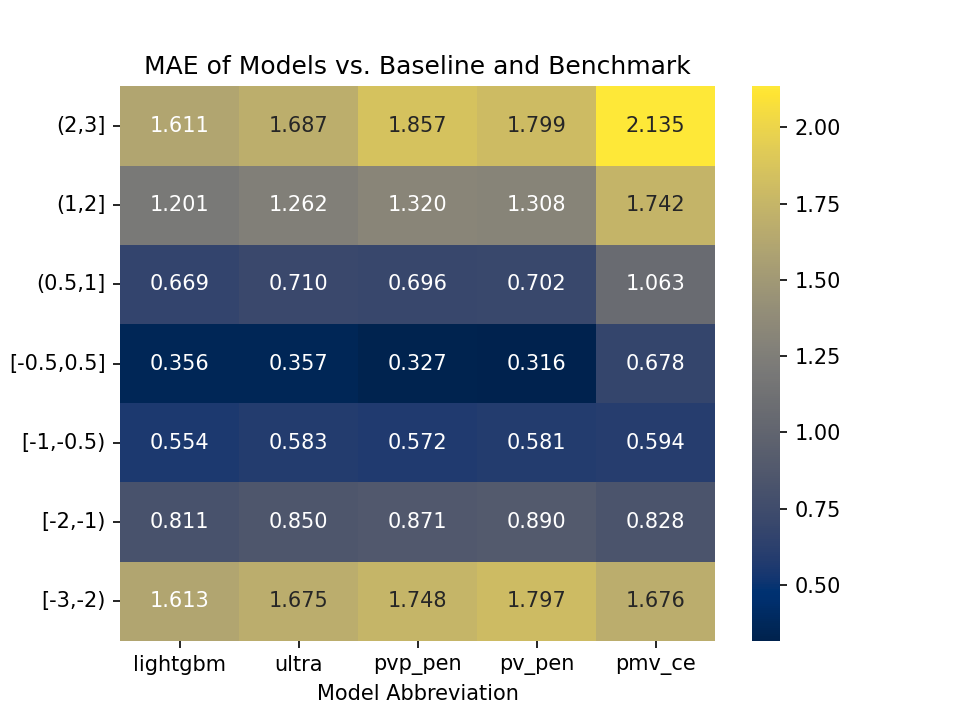
\includegraphics[width=0.49\linewidth]{fig/mods_mae_hm.png}
%     \caption{RMSE and MAE of alternative models tested vs Baseline (PMV\_CE) and Benchmark (lightgbm)}
%     \label{fig:enter-label}
% \end{figure}
To beteter visualize how each model fared within each of the thermal sensation bins, we create a boxen plot across various thermal sensation bins as shown in Figure~\ref{fig:residual-boxen} to compare their respective residuals against each other.
\begin{figure}[h!]
    \centering
    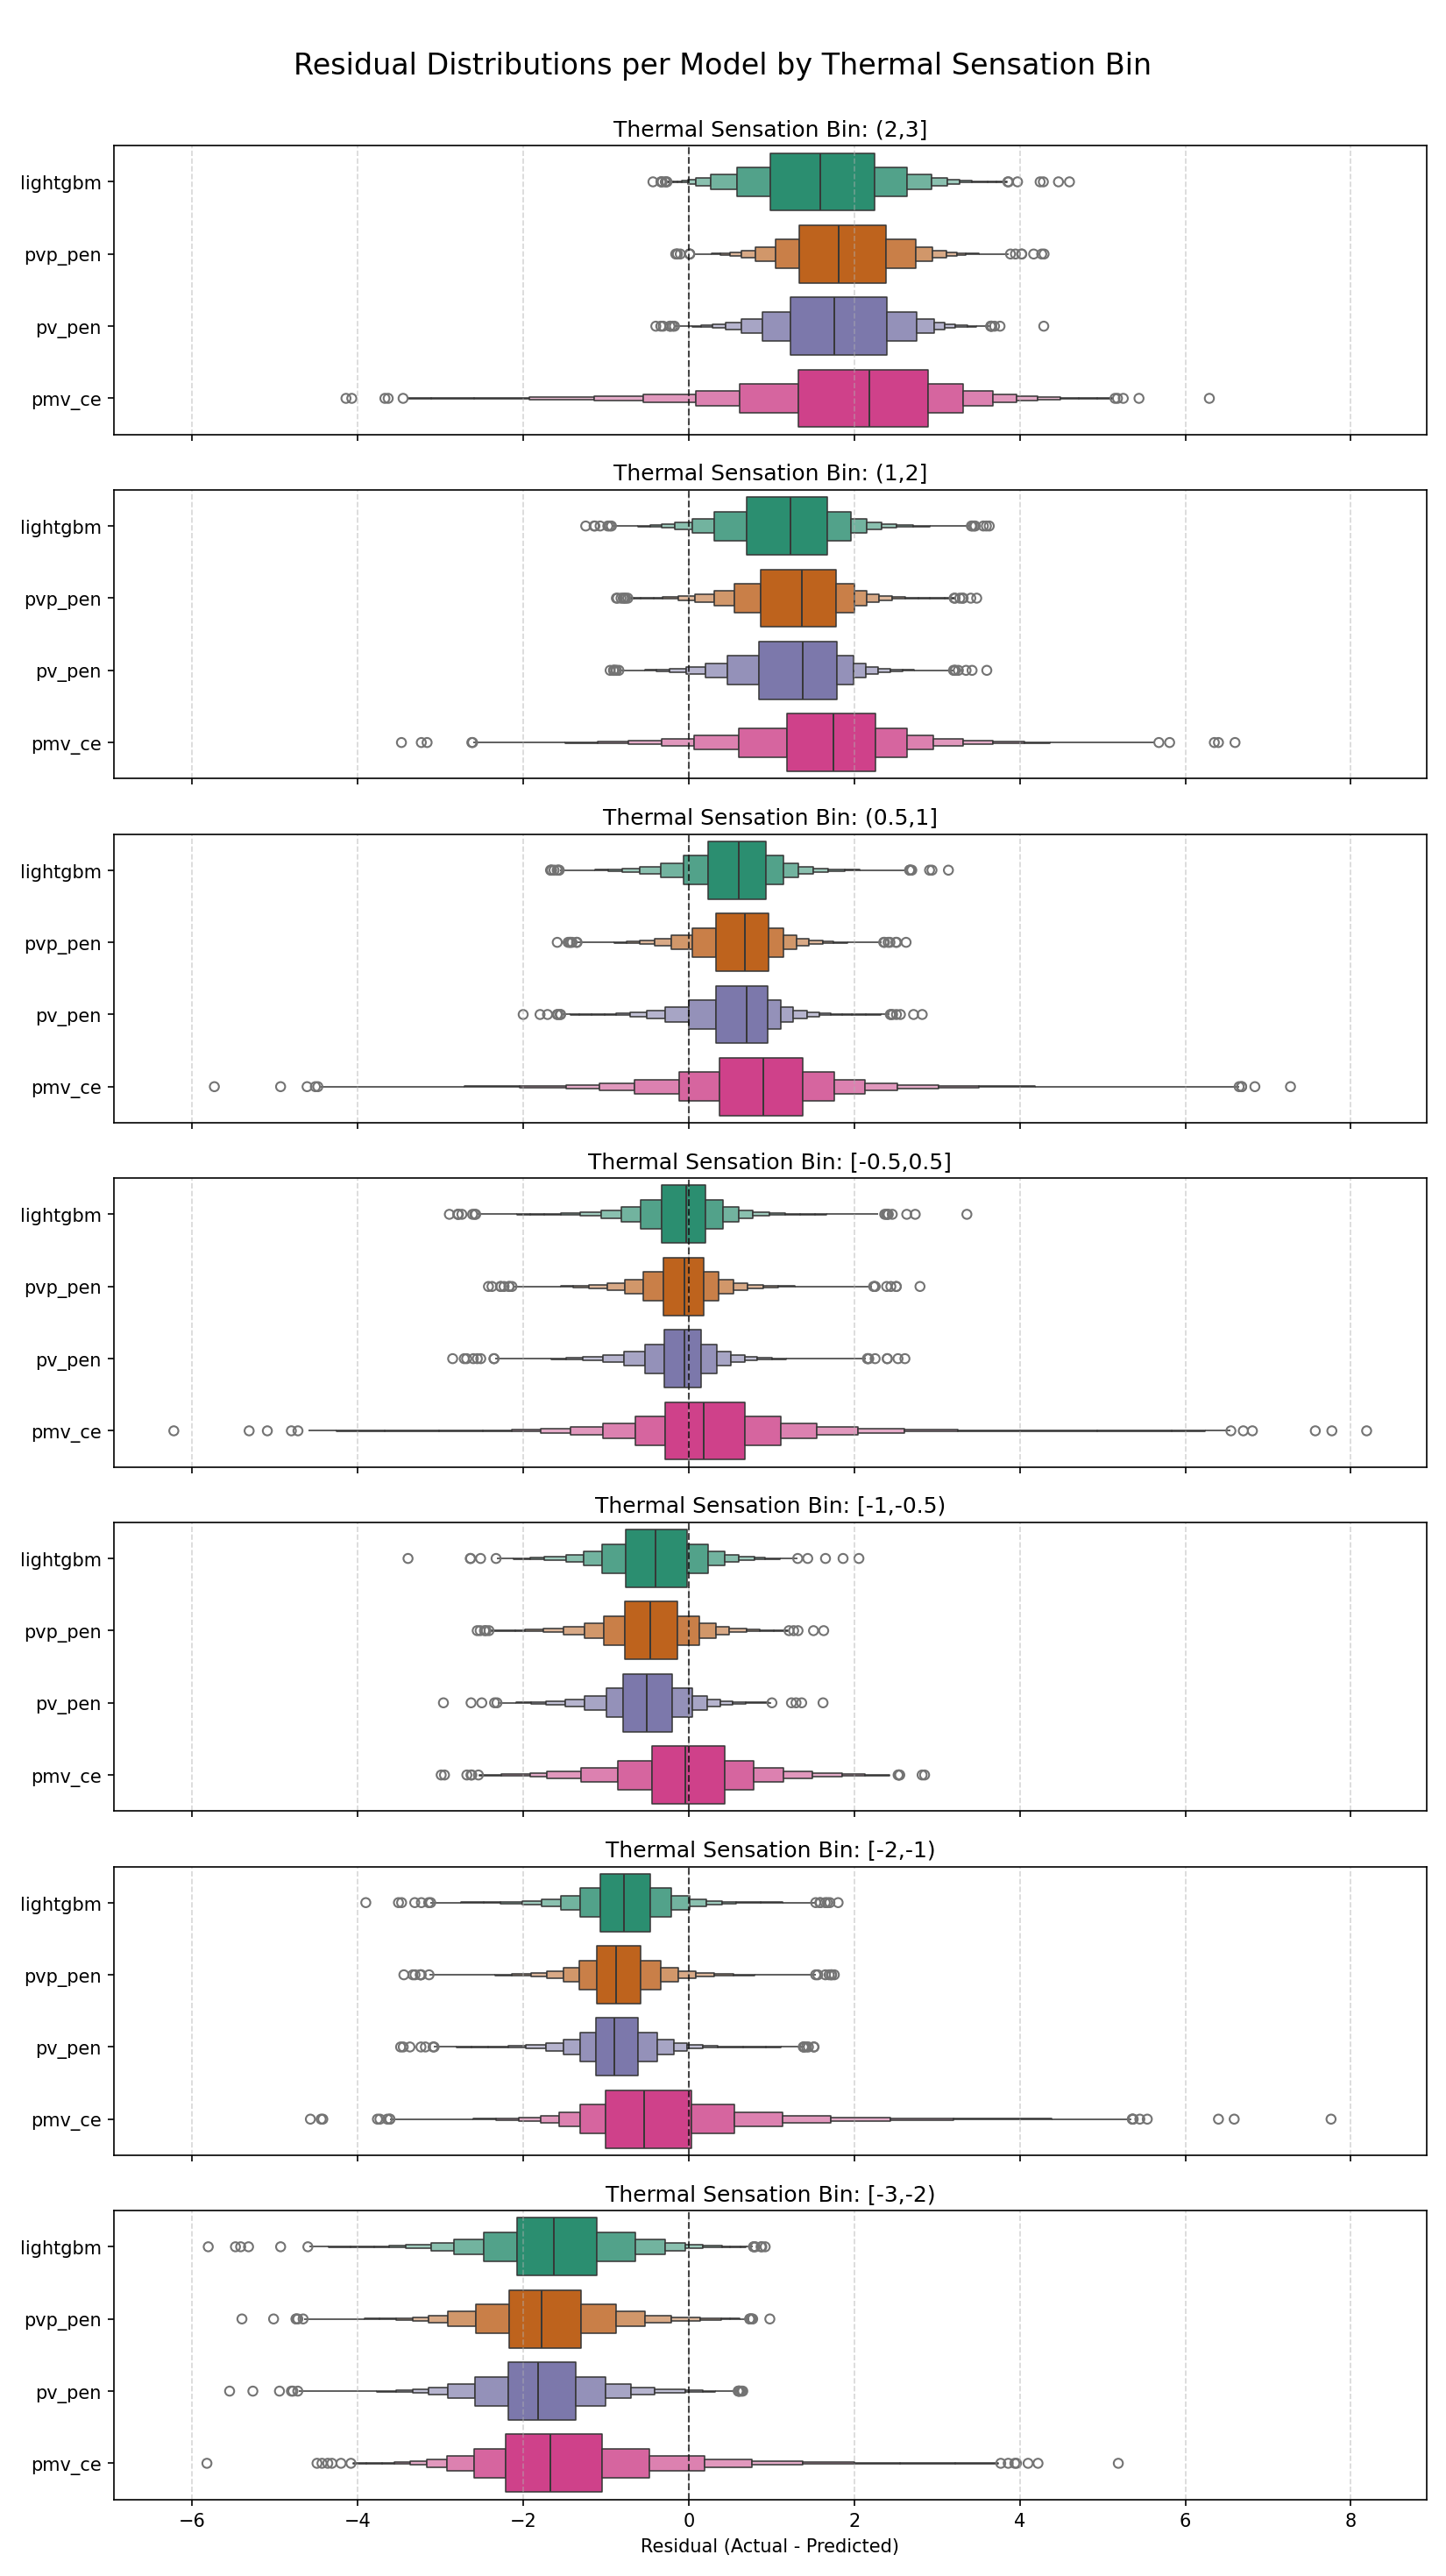
\includegraphics[width=0.55\linewidth]{fig/res_boxen.png}
    \caption{Residuals from models measured}
    \label{fig:residual-boxen}
\end{figure}

Qualitatively, the distribution of residuals ocross different models can be simply compared against one another where lightgbm, despite its accuracy tends to result in a much wider range of prediction resituals, which is adequately modulated by our proposed PINN-framework across the two model alternatives. 

\subsubsection{Performance by Fill}
% In the meantime, we also evaluated the performance metrics of the models across different data availaibility `rungs', specifically the percentages of fields that are not null across all raw inputs, divided into 10\% buckets. This leads to Figure~\ref{fig:10perc_metrics}. Similar to the results reported with respect to thermal sensation bins, switching of VAE leads to RMSE and MAE increase across all levels of not-null values. Across the various percentage fill buckets reported in Figure~\ref{fig:10perc_metrics}, this translates to an average 31.5\% and 28.2\% of RMSE and MAE increase from lightgbm as the benchmark model. By incorporating the PINN framework, the RMSE and MAE increase dropped to 4.7\% and 5.1\% respectively, which ultimately dropped to 3.4\% and 3.9\% for the final lightGBM model leveraging the imputed dataset.%Expand a little...? 

Analyzing model performance across different levels of data completeness, stratified by the percentage of non-null input features per record (Figure~\ref{fig:10perc_metrics}), reveals expected trends. As illustrated by the heatmaps for RMSE and MAE, the predictive accuracy of all models generally degrades as the data fill percentage decreases. For instance, the PINN-VAE models (pv\_pen, pvp\_pen) show increased error metrics in the 40-60\% fill range compared to the >90\% fill range. This observed degradation is likely attributable to the fundamentally reduced information content available for prediction in records with higher missingness. Key variables, including the personal data required for reliable BMR calculations (\texttt{age}, \texttt{height}, \texttt{weight}) and potentially other influential environmental or contextual factors, are more frequently absent in these lower-fill data rows. This inherent lack of crucial input information naturally limits the predictive capability achievable by any modeling approach. Nonetheless, the PINN-VAE models consistently outperformed the unconstrained VAE across all fill levels and maintained performance closer to the LightGBM benchmark, particularly at higher fill percentages.


\begin{figure}[h!]
    \centering
    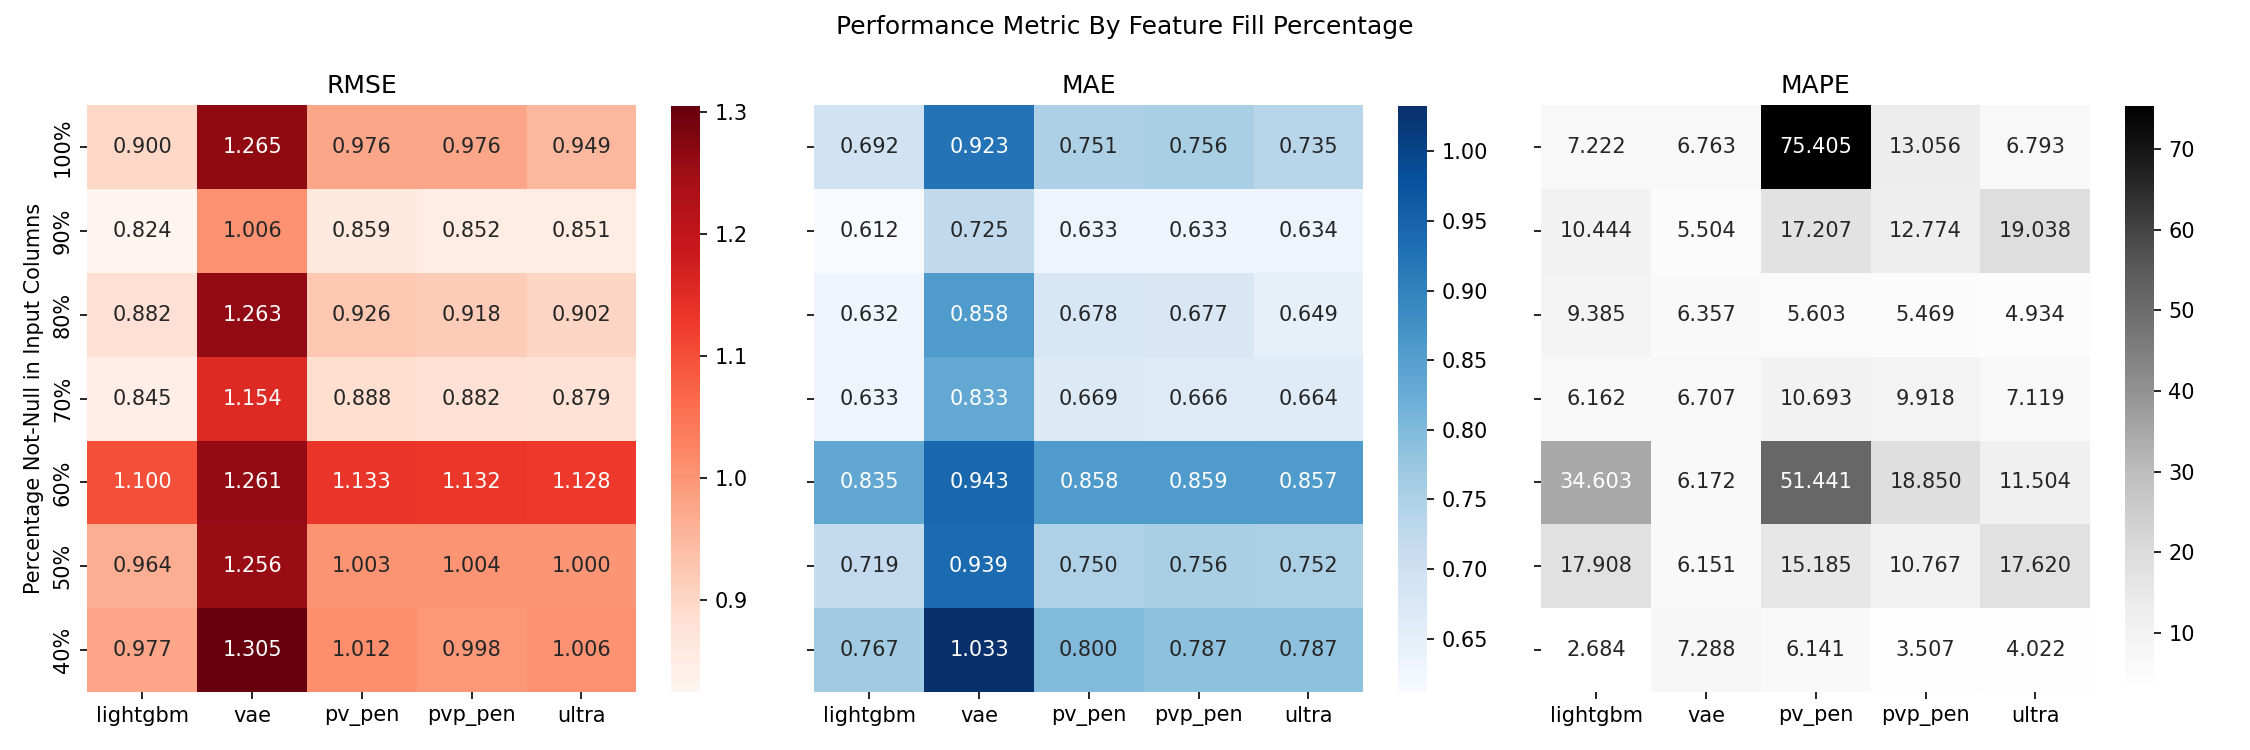
\includegraphics[width=0.99\linewidth]{fig/PerfMetrics_10.png}
    \caption{Root mean squared error (left), mean absolute error (middle) and mean absolute percentage error across all models evaluated}
    \label{fig:10perc_metrics}
\end{figure}
\subsubsection{Around Thermal Neutral Zone}%Does this belong to discussion...?

We had already seen that both PINN-based models were noticeably more precise than LightGBM inside the neutral zone, but a single RMSE does not show why. 
%%%%???
The results we got are as Table~\ref{tab:dir_penalty}. 

\begin{table}[t]
\centering
\caption{Direction-penalty metric  
$\Delta_{\text{dir}}=\text{MAE}_{\text{wrong sign}}-\text{MAE}_{\text{right sign}}$  
(lower is better; a positive value means the model’s error grows once it crosses to the wrong side of neutral).
Bootstrapped 95\,\% confidence intervals are based on 1\,000 resamples of the
out-of-sample rows produced by the original 5-fold CV.}
\label{tab:dir_penalty}
\begin{tabular}{lcc}
\toprule
\textbf{Model} & $\boldsymbol{\Delta_{\text{dir}}}$ & 95\,\% CI \\ 
\hline
PMV\textsubscript{CE}            & 0.1236 & [\,0.1130,\;0.1333\,] \\
LightGBM              & 0.0459 & [\,0.0386,\;0.0530\,] \\
VAE                   & $-0.1565$ & [\,-0.1657,\;-0.1470\,] \\
PINN–VAE (\texttt{pv\_pen})      & $-0.0036$ & [\,$-0.0112$,\;0.0035\,] \\
PINN–VAE–PPI (\texttt{pvp\_pen}) & $-0.0181$ & [\,$-0.0250$,\;$-0.0108$\,] \\
Ultra LightGBM (\texttt{ultra})  & 0.0342 & [\,0.0273,\;0.0409\,] \\

\bottomrule
\end{tabular}\label{tb:neutral-pen}
\end{table}

According to Table~\ref{tab:dir_penalty}, LightGBM and PMV\textsubscript{CE} incur clear asymmetric costs ($\approx$0.05 and 0.12 votes, respectively), meaning their errors inflate sharply when they cross neutral.
The physiology-guided networks behave differently: the plain PINN-VAE shows no significant asymmetry (CI straddles zero), and the PINN-VAE–PPI variant actually drives the wrong-sign error \emph{below} the right-sign error by $\approx$0.02 votes. Inspecting results from the table we noticed the performance of PINN-VAE was effective in a few interesting ways:

\paragraph{PINN variants level the playing field.}  
  With the physiology constraint—and particularly when the PPI gate is used—errors remain tightly bounded even if the network picks the wrong side of neutral.  We acknowledge the negative $\Delta$ may sound counter-intuitive, but it simply means the model’s over- and under-shoots have similar magnitudes.

\paragraph{LightGBM and PMV are asymmetric.}  
  Their right-sign mistakes are modest, but once they cross the neutral point the error grows by 0.03–0.12 votes, a pattern that matches occupant complaints about “getting the sign wrong.”  For control applications a small symmetric error is preferable: the HVAC system can compensate with a fixed offset.  Large asymmetric errors, by contrast, cause abrupt, perception-opposite responses.

To put the table into a better perspective, we also visually broke down the performance change with Figure~\ref{fig:neu_zone}. The improvement of RMSE of VAE observed in the thermal neutral zone in ~\ref{fig:rmse-7bucket} gets borken down clearly with 

\begin{figure}[h!]
    \centering
    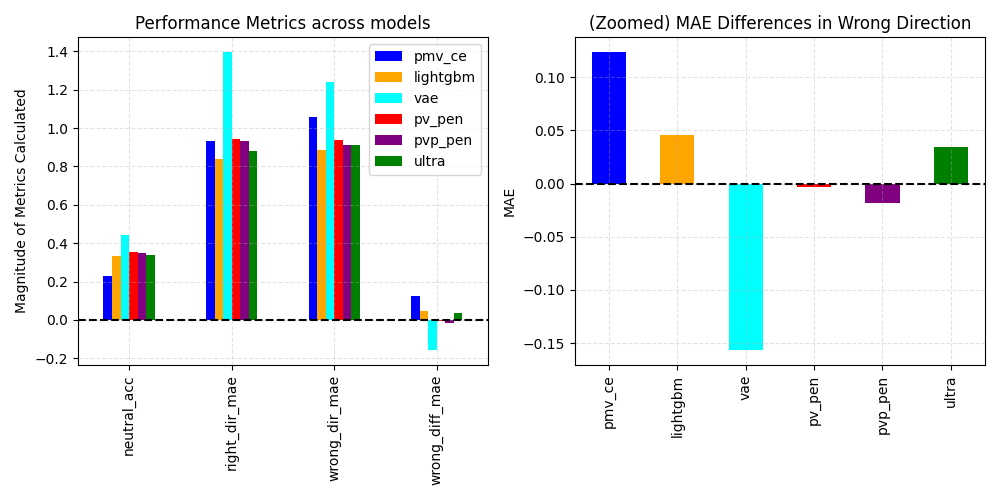
\includegraphics[width=0.95\linewidth]{fig/w5_dir.png}
    \caption{Neutral Zone Performance Lift Analysis: Zone-specific accuracy, MAE of correct/wrong direction and their respective differences}
    \label{fig:neu_zone}
\end{figure}

This analysis using the direction-penalty statistic, $\Delta_{dir} = \text{MAE}_{\text{wrong sign}} - \text{MAE}_{\text{right sign}}$, reveals distinct behaviors near the thermal neutral zone ($|TSV| \le 0.5$). As shown in Table~\ref{tb:neutral-pen}, baseline models like $PMV_{CE}$ and LightGBM exhibit significantly positive $\Delta_{dir}$ values, indicating that their prediction errors substantially increase when the predicted sensation incorrectly crosses the neutral threshold (i.e., predicting warm when the true sensation is cool, or vice-versa). In contrast, the physiology-guided networks demonstrate markedly different behavior. The PINN-VAE (pv\_pen) shows no significant asymmetry ($\Delta_{dir} \approx -0.004$, with a 95\% CI spanning zero), while the PINN-VAE-PPI (pvp\_pen) achieves a slightly negative $\Delta_{dir}$ ($\approx -0.018$). This indicates that, for the PINN-based models, the magnitude of prediction error remains tightly bounded and symmetric, regardless of whether the prediction falls on the correct or incorrect side of neutral. This behavior, attributed to the physiological constraints preventing unrealistic predictions, is highly desirable for control applications where large, asymmetric errors can lead to inappropriate system responses\cite{Jain2018}. The PINN framework effectively removes the sharp performance cliff observed in traditional models when they misjudge the direction of thermal sensation relative to neutral.

Thus, adding the physiological loss—and, when available, the personal-profile embedding—not only improves overall RMSE but also removes the sharp performance cliff that traditional models hit when they guess the wrong side of comfort.

\subsection{Imputed Features from VAE Architecture}
A key capability of the VAE framework is data imputation. We qualitatively assessed the imputed distributions for variables with high initial missingness, namely \texttt{age}, \texttt{height}, and \texttt{weight} (Figure~\ref{fig:impu_three}), as well as the intermediate physiological variable $\hat{T}_{skin}$ (Figure~\ref{fig:skin_inputs}). Visual inspection reveals that the PINN-VAE produces more plausible distributions compared to an unconstrained VAE, avoiding unrealistic values (e.g., age < 0, height < 100 cm) due to the implicit guidance from the learned data structure and explicit physiological constraints.

While Table~\ref{tab:performance_updated} shows that LightGBM and PINN-VAE models achieve superior performance metrics, it is particularly notable that the unconstrained VAE performs the worst across all evaluation criteria—despite having access to the same data and architecture depth. This underperformance confirms that imputation alone, without physiological regularization, is insufficient for meaningful TSV prediction. The poor performance of VAE, despite its flexibility, highlights the importance of constraining intermediate outputs through biophysical priors. The improvement in PINN-VAE and further gains in PINN-VAE–PPI validate the necessity of combining imputation and physiological structure.


\begin{figure}[h!]
    \centering
    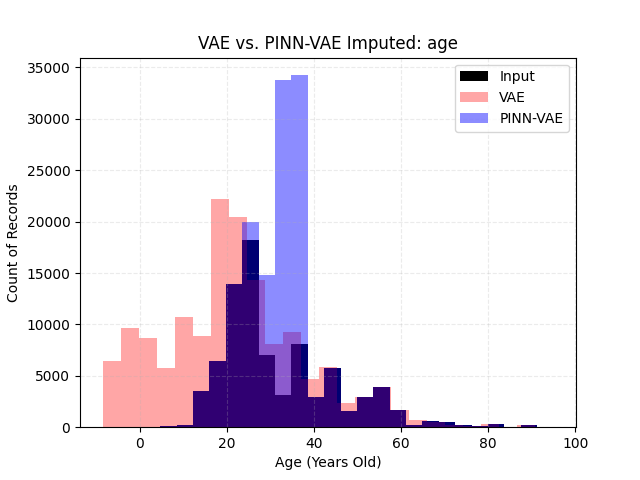
\includegraphics[width=0.5\linewidth]{fig/imp_age.png}
    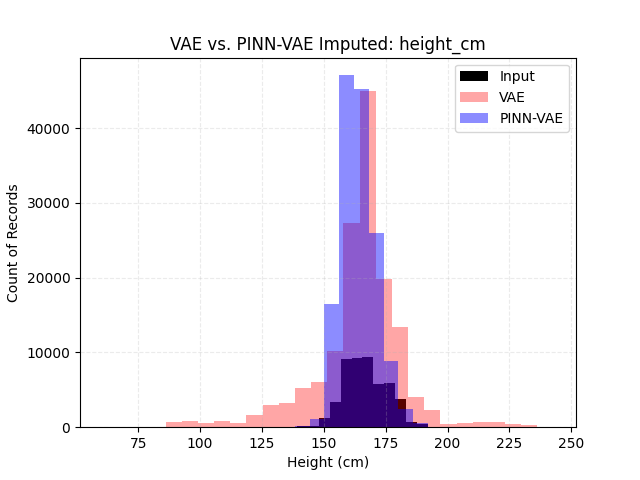
\includegraphics[width=0.5\linewidth]{fig/imp_height_cm.png}
    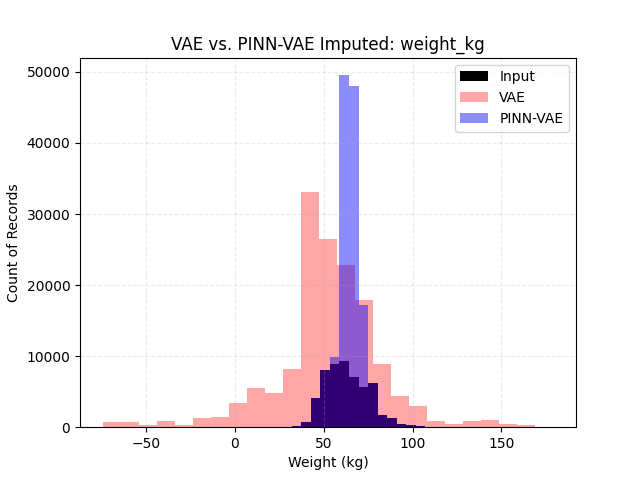
\includegraphics[width=0.5\linewidth]{fig/imp_weight_kg.png}
    \caption{Imputed age, height and weight field values histogram between simple VAE and PINN-VAE}
    \label{fig:impu_three}
\end{figure}
Quantitative evaluation of imputation accuracy (e.g., calculating RMSE or MAE between imputed values and ground-truth values on a held-out test set) was not performed in this study. The primary variables requiring the most imputation (\texttt{age}, \texttt{height}, \texttt{weight}) originally suffered from very high levels of missing data (up to 70\%), leaving insufficient reliable ground-truth data within the dataset to conduct a robust quantitative validation of imputation performance for these specific fields. Furthermore, optimizing imputation accuracy itself, for instance through comparisons involving artificial data masking, was considered secondary to the main research objective of evaluating the overall PINN-VAE framework for constrained prediction in the presence of missing data. A dedicated study focusing on quantitatively optimizing and validating imputation strategies for these specific variables could be a valuable direction for future work.

Similarly, a quantitative comparison quantifying the frequency of physiological constraint violations in imputed intermediate variables ($\hat{T}_{core}, \hat{T}_{skin}, \hat{w}$) between the constrained PINN-VAE and an unconstrained VAE was not conducted. This is primarily due to the lack of comprehensive ground-truth physiological measurements in the original aggregated dataset; the 'input' physiological values used for comparison were themselves derived from Gagge's model \cite{gagge1986standard}. The analysis therefore focused on the qualitative demonstration, via imputed distributions (Figure~\ref{fig:impu_three}), that the physics-informed constraints effectively guide the imputation process towards generating more physiologically realistic values compared to an unconstrained approach.

As was outlined in the methodology, we employed a soft constraint on the imputation of the age, height and weight columns. Our imputed values for the three fields becomes much more reasonable in terms of coverage of values in contrast to age below 0 years old and height below 100 centimeters, and weight below 0 kg etc. Visually examining the VAE against the PINN-VAE results for these fields where null values are commonly observed, PINN-VAE does appear to be providing a much more reasonable imputation quality. %Expand further?

Beyond qualitatively comparing the results of imputed data of the combined dataset, we also compared the intermediate outputs of $T_{skin}$ as outlined in methodology to assess how PINN-VAE framework affects the resulting intermediate outputs of our proposed framework. Recognizing that $T_{skin}$ were initially calculated with analytical equations developed by Gagge et al. following their built-in assumptions, it is important to point out that its original inputs may need to be further confined. We also want to point out that, while direct quantitative validation of imputation accuracy for variables like age or height was precluded by the high degree of initial missingness, the qualitative plausibility demonstrated (Figure~\ref{fig:skin_inputs}) and the improved downstream predictive performance compared to an unconstrained VAE support the effectiveness of the constrained imputation within the overall framework's objectives.
\begin{figure}[h!]
    \centering
    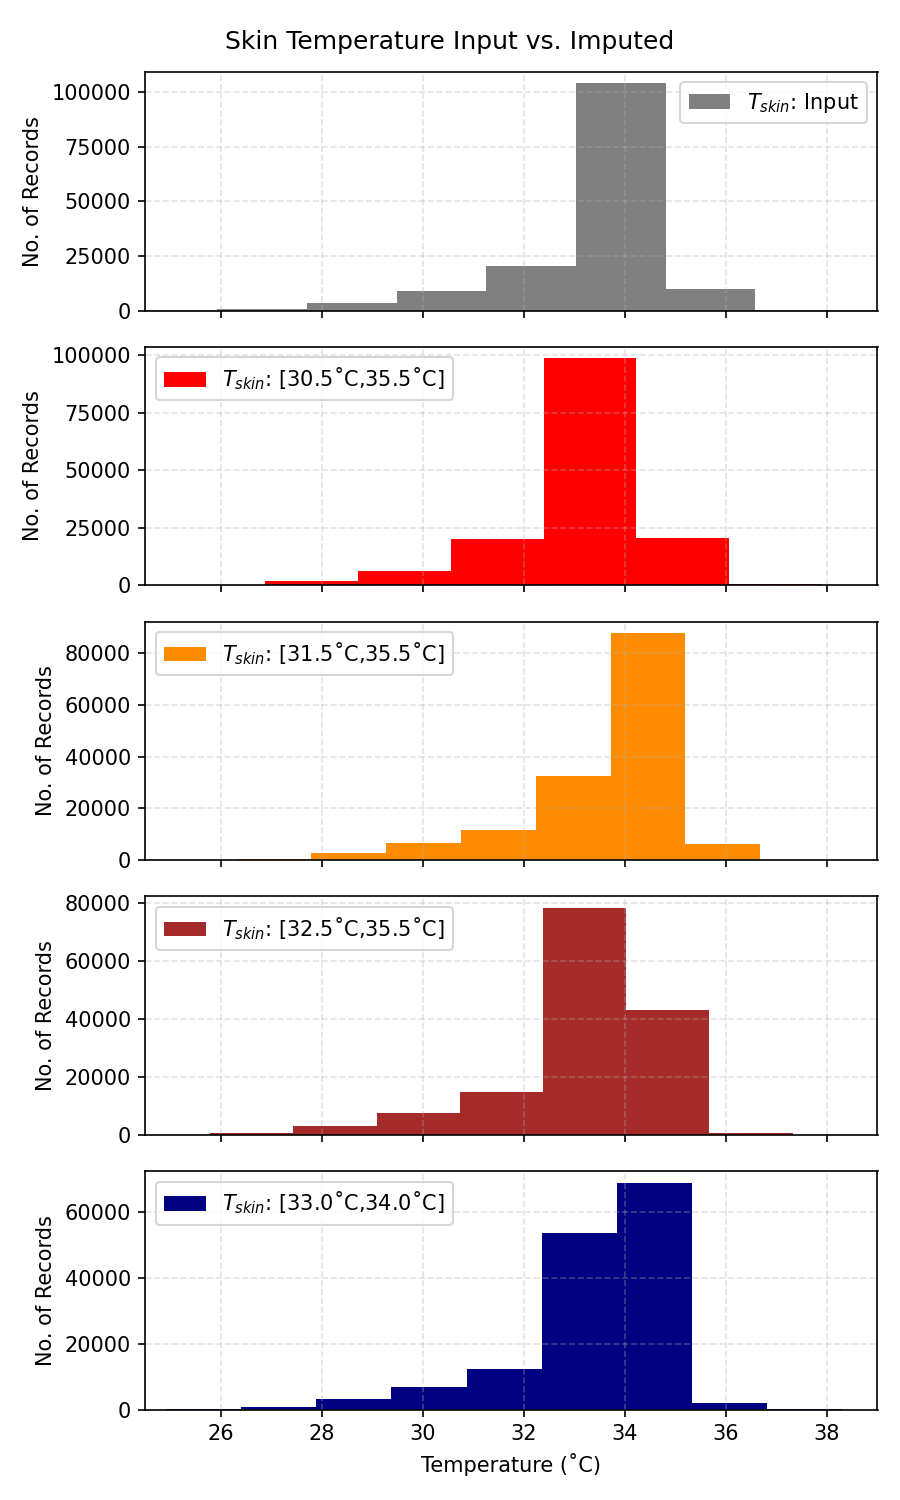
\includegraphics[width=0.45\linewidth]{fig/skinimput.png}
    \caption{Imputed Skin temperature with different skin temperature penalty settings ranging from 30.5$\degree$ C to 35.5 $\degree$ C}
    \label{fig:skin_inputs}
\end{figure}


Figure~\ref{fig:skin_inputs} further illustrates the model's thermoregulatory response by showing the distribution of the imputed intermediate variable $\hat{T}_{\text{skin}}$ under progressively narrower soft constraints. The initial physiological constraint applied a range of $[30, 36]^{\circ}$C. As depicted in the subsequent panels of Figure 11, when this range was incrementally narrowed (from $[30.5, 35.5]^{\circ}$C down to $[33.0, 34.0]^{\circ}$C), the resulting distribution of imputed $\hat{T}_{\text{skin}}$ shifted and became more concentrated. This demonstrates a unique, non-linear relationship where tightening the soft constraint on skin temperature directly influences the model's imputed physiological state. While a similar analysis for $\hat{T}_{\text{core}}$ is not presented, its predicted values remained tightly clustered within physiologically plausible bounds (constrained between $[36, 38]^{\circ}$C), reflecting the body's stricter core temperature regulation. Nonetheless, the observed modulation of $\hat{T}_{\text{skin}}$ distribution based on its constraints highlights the effective physiological regulation capability embedded within the proposed PINN-VAE framework, where adjustments in one physiological parameter influence the overall predicted state.